%-----------------------------------------------------------------------
% Functional Programming 4
% John O'Donnell, Wim Vanderbauwhede
% University of Glasgow
%-----------------------------------------------------------------------

\documentclass{beamer}
\usepackage{jtodlecseriesFP4}

% Identify this presentation
\SetPresentationTitle
  {Computations and Types}
  {Computations and Types}
\SetPresentationNumber
  {6}
\SetPresentationDate
  {Week 3-2}
  {Week 3-2}

%-----------------------------------------------------------------------
% Beginning

\begin{document}

\begin{frame}
  \PresentationTitleSlide
\end{frame}

\begin{frame}
  \frametitle{Topics}
  \tableofcontents
\end{frame}

%-----------------------------------------------------------------------
\begin{frame}[fragile]
\begin{center}
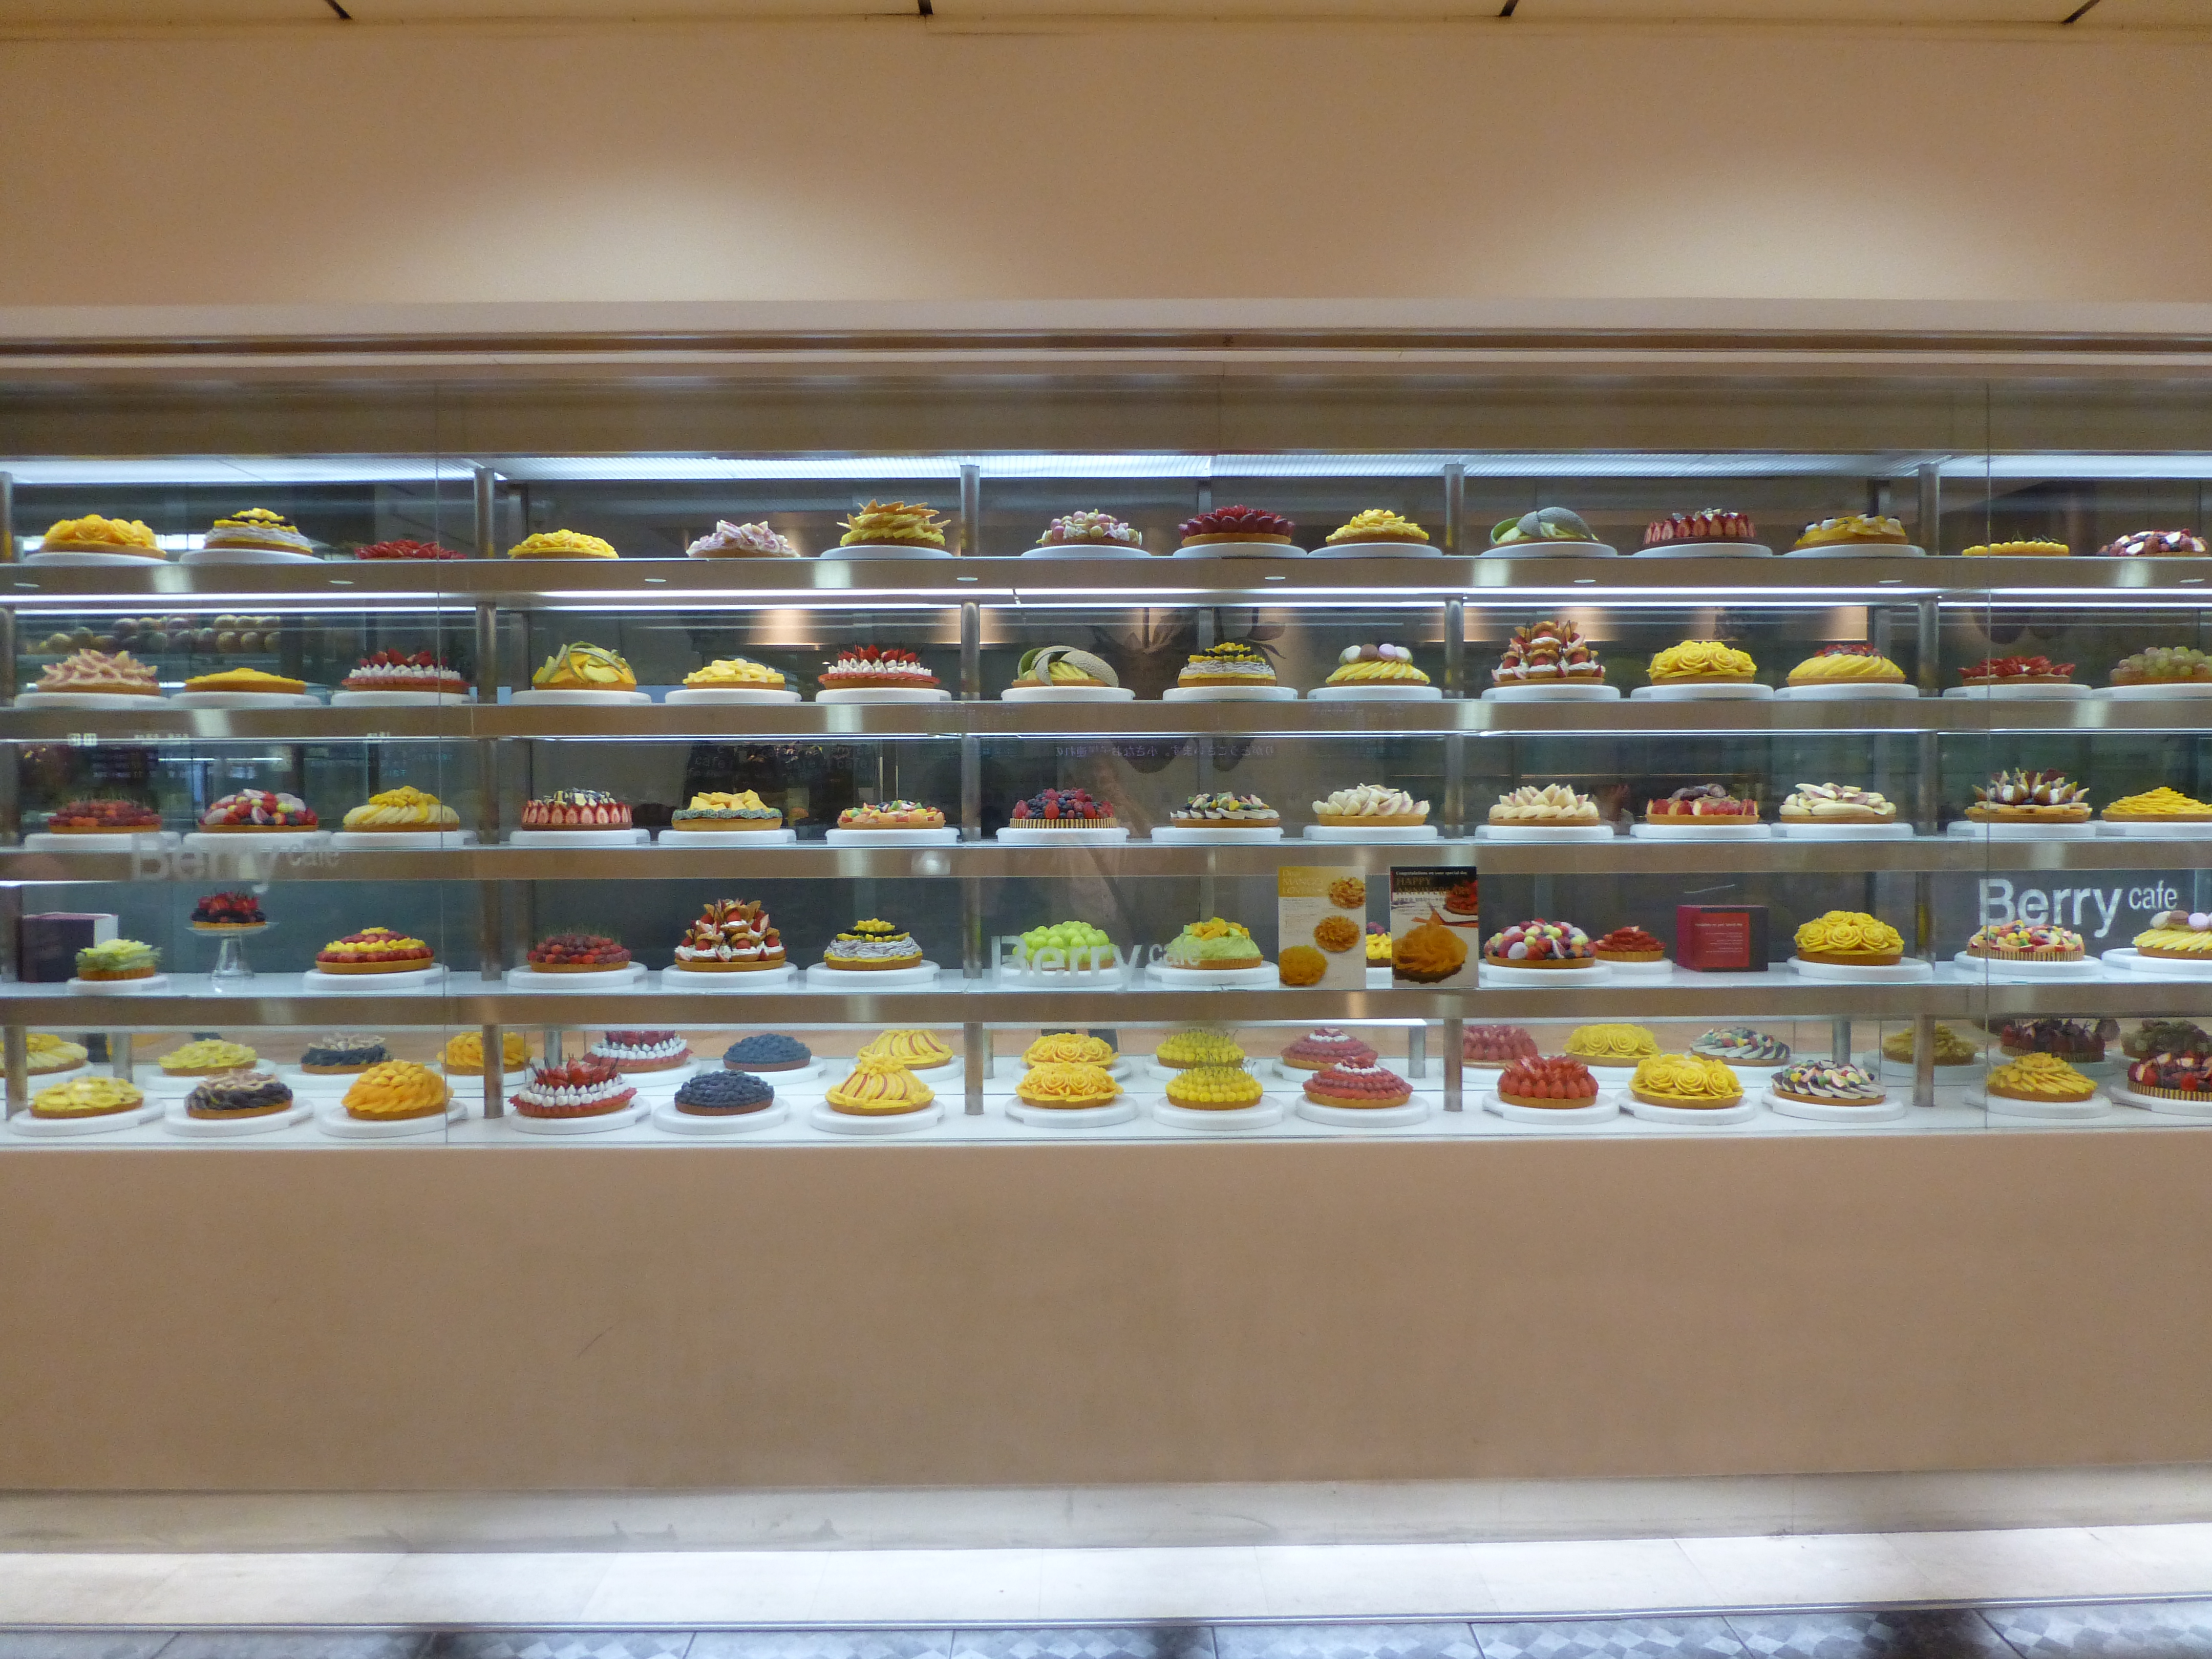
\includegraphics[scale=0.075]
    {figures/jpg/pic08.jpg}
\end{center}
\end{frame}
%-----------------------------------------------------------------------
\section{IO Operations }

%-----------------------------------------------------------------------
\subsection{Computations}

\begin{frame}
\frametitle{Computations}

\begin{itemize}
\item Most programming languages have types for primitive data:
  $Int$, $Bool$, $Double$, $Char$.
\item Most languages also have at least a few types for structured
  data, such as arrays.  (Haskell has this.)
\item Some languages go farther, and have types for more advanced
  data structures: tuples, lists, records, enumerations.  (Haskell
  has all these.)
\item A few languages go still farther, and have user-definable
  types for general structures like trees and graphs.  (Haskell has
  this.)
\item Haskell goes still farther: it has the concept of a
  \emph{computation}, and \emph{types to represent computations}.
\item Computations are ``first class'': they can be used as
  arguments to functions, or results of functions, they can be
  stored in data structures, etc.
\end{itemize}

\end{frame}

%-----------------------------------------------------------------------
\begin{frame}[fragile]
\frametitle{Computation types}

\begin{itemize}
\item A computation type has a form like $IO\,Int$.
  \begin{itemize}
  \item The first part, $IO$, is a \emph{monad}.  We'll look at
    monads later, but for now, think of a monad as the method by
    which the computations in a $do$ expression are combined into a
    larger computation.
  \item There are many monads in Haskell, and you can define your
    own.  For the time being, we will be working with just one
    monad --- $IO$ --- so all our computations will have types that
    start with $IO$.
  \item The second part ($Int$ in the example above) is the type of
    \emph{the result computed by the computation}.
  \end{itemize}
\item So $IO\,Int$ means ``the type of a computation that does some
  work and then eventually produces a value of type $Int$''.
\end{itemize}

\end{frame}

%-----------------------------------------------------------------------
\begin{frame}[fragile]
\frametitle{The type of $putStrLn$}

Here is the type of $putStrLn$.  It isn't a statement!  It's a
function that takes an argument and returns a result.

\begin{verbatim}
putStrLn :: String -> IO ()
\end{verbatim}

\begin{itemize}
\item $putStrLn$ takes a $String$ and it returns a computation.
  That computation has type $IO ()$.
\item The computation must run in the $IO$ monad.  This means you
  can combine $putStrLn$ with other $IO$ operations, but not with
  some completely unrelated computations that we'll encounter
  later.
\item When the computation executes it will perform the output.  It
  doesn't have a useful result to produce, so by convention it just
  produces the empty tuple $()$.
\item The application $putStrLn$\emph{ "hello"} has type $IO\, ()$ --- when
  you apply the function $putStrLn$ to a string, the result is the
  computation.
\end{itemize}

\end{frame}

%-----------------------------------------------------------------------
\begin{frame}[fragile]
\frametitle{Some text output operations}

\begin{itemize}
\item $putStr :: String -> IO ()$
\item $putStrLn :: String -> IO ()$
\item $putChar :: Char -> IO ()$
\end{itemize}

\end{frame}

%-----------------------------------------------------------------------
\begin{frame}[fragile]
\frametitle{$getChar$}

Here is the type of $getChar$:

\begin{verbatim}
getChar :: IO Char
\end{verbatim}

\begin{itemize}
\item $getChar$ is not a function: it doesn't need an arguments to
  tell it how to read a character.
\item It is simply a constant, like $42$ or $'a'$ or any other
  constant.
\item The type says that
  \begin{itemize}
  \item $getChar$ executes in the $IO$ monad --- that means that
    you can combine it in a $do$ expression with other $IO$
    operations, but not with operations that are completely
    unrelated.
  \item When the computation is executed, it yields a result with
    type $Char$.
  \end{itemize}
\end{itemize}
\end{frame}

%-----------------------------------------------------------------------
\begin{frame}[fragile]
\frametitle{Receiving the result of a computation}

\begin{itemize}
\item When the computation $getChar$ is executed, we need to grab
  the result so we can use it!
\item This is done by binding a name to the result of the computation.
\item $c \leftarrow getChar$ means ``run the computation $getChar$ and then
  define $c$ to be the value produced by the computation''.
\item Since $getChar :: IO Char$, we will have $c :: Char$
\item In general, if you write $x  \leftarrow someComputation$, where
  $someComputation :: IO a$ for any type $a$, then $x$ will have
  the type $a$.
\end{itemize}

\end{frame}

%-----------------------------------------------------------------------
\begin{frame}[fragile]
\frametitle{More text input operations}

\begin{itemize}
\item $getChar :: IO Char$
\item $getLine :: IO String$
\end{itemize}

\end{frame}



%-----------------------------------------------------------------------
\subsection{Using let  in a monad}
\begin{frame}[fragile]
\frametitle{Using \emph{let} in a monad}

\begin{itemize}
\item What if you want to do something ordinary in a $do$
  expression, like just say $x = 2+2$?
\item You can't put an equation like this in a $do$ expression
  because it doesn't have the right monadic type.
\item Instead, you write $let\, x = 2+2$.  This is now a computation,
  and the types are ok.
\item A typical $do$ expression combines computations (with and
  without $\leftarrow$ and $let$ expressions.
\end{itemize}

\end{frame}

%-----------------------------------------------------------------------
\subsection{show and read}

\begin{frame}[fragile]
\frametitle{The $show$ function}

\begin{itemize}
\item When you have done some calculation (like $2+2$) you may want
  to print it!
\item But $putStrLn$ requires a $String$ to print, and $2+2 :: Int$.
\item Solution: you can apply the function $show$ to an $Int$, and
  it converts it to a string.
\end{itemize}

\begin{verbatim}
show (2+2) --> "4"
\end{verbatim}

\emph{Note that the result is a string, not a number.}

\end{frame}

%-----------------------------------------------------------------------
\begin{frame}[fragile]
\frametitle{The $read$ function}

\begin{itemize}
\item When you have read some input with $getLine$, it is a
  $String$.
\item You can convert it to an $Int$ (or some other type) using
  $read$.
\item But if you have read a string like "23", how can $read$ know
  whether it should give you an $Int$, or a $Double$, or one of the
  many other types it could be?
\item \emph{You need to tell it} by specifying the type of the
  result $read$ should produce.
\end{itemize}

\begin{verbatim}
read "23" :: Int     --> 23
read "23" :: Double  --> 23.0
\end{verbatim}

If you just write $read\; "23"$ Haskell will give an error message,
referring to ``Ambiguous type variable $\ldots$''.

\end{frame}

%-----------------------------------------------------------------------
\begin{frame}[fragile]
\frametitle{Example: program 'Lec04Prog1.hs'}

\begin{verbatim}
main =
  do  putStrLn "Enter a number"
      xs <- getLine
      let n = 3 * (read xs :: Int)
      putStrLn (show n)
\end{verbatim}

\begin{verbatim}
*Main> main
Enter a number
21
63
\end{verbatim}

\end{frame}

\section{Algebraic data types}
\begin{frame}
\frametitle{Algebraic data types}

\begin{itemize}
\item The fundamental mechanism for defining data structures in
  Haskell is \emph{algebraic data types}
  \begin{itemize}
  \item Don't confuse these with abstract data types.  Haskell has
    those too, and they are quite different.
  \item It isn't a good idea to use the acronym ADT---someone is
    sure to misunderstand you.
  \end{itemize}
\end{itemize}

\end{frame}

%-----------------------------------------------------------------------
\begin{frame}
\frametitle{Form of an algebraic data type}

\begin{itemize}
\item Define the type with a \texttt{data} declaration
\item There are one or more alternatives separated by $\mid$
\item Each alternative starts with a \emph{constructor}, a name
  that must begin with an upper case letter, followed by zero or
  more types of the fields
\item The algebraic data type may be just a monomorphic type
  (e.g. \texttt{Bool} or \texttt{Foo}) or it may be polymorphic (e.g. \texttt{Tree a b}).
\end{itemize}

\end{frame}

%-----------------------------------------------------------------------
\begin{frame}[fragile]
\frametitle{Bool is just an algebraic data type}

Bool is defined in the standard libraries:

\begin{verbatim}
data Bool = False | True
\end{verbatim}

\end{frame}

%-----------------------------------------------------------------------
\begin{frame}[fragile]
\frametitle{Tuples are algebraic data types with sugar}

We could define tuples like this:

\begin{verbatim}
data Pair a b = Pair a b           -- (a,b)
data Triple a b c = Triple a b c   -- (a,b,c)
\end{verbatim}

That's essentially the way tuples are implemented in Haskell,
except that there is ``syntactic sugar'' so you can write \texttt{(a,b)}
rather than \texttt{Pair a b}.

\end{frame}

%-----------------------------------------------------------------------
\begin{frame}[fragile]
\frametitle{Record syntax for tuples}

To make access to tuple fields convient, Haskell provides a record syntax. For example, the type for the F95 variable declaration in the coursework is:

\begin{verbatim}
data VarDecl = MkVarDecl {
   vd_vartype :: VarType
  ,vd_dimension :: [Range]	
  ,vd_intent :: Intent
  ,vd_varlist :: [VarName]
  ,vd_argmode :: OclArgMode
  ,vd_is_arg :: Bool
} 
-- Assuming var_decl is defined:
is_arg :: Bool  = vd_is_arg var_decl 
var_decl' :: VarDecl  = var_decl{vd_is_arg = True}

\end{verbatim}



\end{frame}

%-----------------------------------------------------------------------
\begin{frame}[fragile]
\frametitle{Trees}

\begin{itemize}
\item There are many different kinds of trees, so we really don't
  want to pick just one form, turn it into a built-in feature of
  the language, and force programmers to shoe-horn all their own
  data structures into this form.
\item Trees are easy to define using algebraic data types
\item Warning: each constructor name must be unique (within a
  script file or module)
\end{itemize}

\begin{verbatim}
data BinTreeNum =
    Leaf Int | 
    Node BinTreeNum BinTreeNum
data BinTreeNum = 
   Leaf Int | 
   Node Int BinTreeNum BinTreeNum

data BinTree a = Tip | Node a (BinTree a) (BinTree a)
\end{verbatim}

\end{frame}

%-----------------------------------------------------------------------
%-----------------------------------------------------------------------
%-----------------------------------------------------------------------
\subsection{Deriving Show and Read}

\begin{frame}[fragile]
\frametitle{Deriving Show and Read}

\begin{itemize}
\item \emph{show x} produces a character string representation
  of \emph{x}, and \emph{read str :: a} takes a string representing an object
  of type \emph{a} and gives the actual \emph{a} value.
\item The \emph{show} and \emph{read} functions are defined on primitive
  types.
\item But when we define data structures, we need to be able to
  show and read those as well.
\end{itemize}

\end{frame}


%-----------------------------------------------------------------------
\begin{frame}[fragile]
\frametitle{Defining a binary tree}

Here is a typical definition of a binary tree:

\begin{verbatim}
data BinTree a
  = Tip
  | BinTree a (BinTree a) (BinTree a)
\end{verbatim}

We can define a value in this type:

\begin{verbatim}
tree1 :: BinTree Int
tree1 =
  BinTree 23
    (BinTree 34
      (BinTree 2 Tip Tip)
      Tip)
    (BinTree 17 Tip Tip)
\end{verbatim}

\end{frame}

%-----------------------------------------------------------------------
\subsection{Recursion over a tree}
\begin{frame}[fragile]
\frametitle{Recursion over a tree}

\begin{itemize}
\item Recursion over an algebraic data type is similar to recursion
  over a list.
\item You need one defining equation for each alternative in the
  type definition (lists have two alternatives, so they need two
  equations).
\end{itemize}

\begin{verbatim}
addtree :: BinTree Int -> Int
addtree Tip = 0
addtree (BinTree n x y) = n + addtree x + addtree y
\end{verbatim}

\begin{verbatim}
addtree tree1 ~> 76
\end{verbatim}

\end{frame}

%-----------------------------------------------------------------------
\begin{frame}[fragile]
\frametitle{Trying to print a tree}

Now if we enter |tree1| at the prompt in ghci, it will (1) evaluate
the value, and then (2) apply show to it.

{\footnotesize
\begin{verbatim}
*Main> tree1

<interactive>:1:0:
    No instance for (Show (BinTree Int))
      arising from a use of `print' at <interactive>:1:0-4
    Possible fix: add an instance declaration for (Show (BinTree Int))
    In a stmt of a 'do' expression: print it
\end{verbatim}
}

Unfortunately, \emph{show} isn't defined on a new type that \emph{we}
just defined.

\end{frame}

%-----------------------------------------------------------------------
\begin{frame}[fragile]
\frametitle{Defining a tree with $deriving$}

\begin{verbatim}
data BinTree2 a
  = Tip2
  | BinTree2 a (BinTree2 a) (BinTree2 a)
  deriving (Read, Show)
\end{verbatim}

\begin{verbatim}
tree2 :: BinTree2 Int
tree2 =
  BinTree2 23
    (BinTree2 34
      (BinTree2 2 Tip2 Tip2)
      Tip2)
    (BinTree2 17 Tip2 Tip2)
\end{verbatim}

\end{frame}

%-----------------------------------------------------------------------
\begin{frame}[fragile]
\frametitle{Using show and read}

{\footnotesize
\begin{verbatim}
*Main> tree2
BinTree2 23 (BinTree2 34 (BinTree2 2 Tip2 Tip2) Tip2) (BinTree2 17 Tip2 Tip2)
\end{verbatim}
}

{\footnotesize
\begin{verbatim}
*Main> read "BinTree2 567 Tip2 Tip2" :: BinTree2 Int
BinTree2 567 Tip2 Tip2
\end{verbatim}
}

\end{frame}

%-----------------------------------------------------------------------
\end{document}
